\documentclass[11pt]{article}
\usepackage[margin=1in]{geometry}
\usepackage{graphicx}\usepackage{booktabs}\usepackage{amsmath,amssymb}
\usepackage[table]{xcolor}\usepackage[numbers,sort&compress]{natbib}
\usepackage{enumitem}\usepackage{hyperref}\usepackage[capitalize]{cleveref}
\definecolor{abMist}{HTML}{EAF2F5}
\newcommand{\platform}{Alphabrain Platform}\newcommand{\model}{Alphabrain}
\title{\textbf{Online Reinforcement Learning for VLA (RLT bottleneck)}\\[2pt]\large (standalone preview of one report section)}
\author{AlphaBrain --- X-Lab}\date{\today}
\begin{document}\maketitle
% =============================================================================
% AlphaBrain Technical Report — RL on a frozen-VLA bottleneck (RLT) chapter.
% Algorithm-agnostic, compute-efficient online RL for VLA policies.
% Data: LIBERO-Goal, QwenOFT base, offline 50-ep eval. Numbers verified against
% source eval JSON (see RL_REPORT_DATA_PROVENANCE.md). Honest efficiency framing
% vs large-scale full-VLA RL (RLinf-VLA).
% =============================================================================
\newcommand{\sotbd}{\textcolor{black!35}{$\dagger$}} % multi-seed n=3 complete (seeds 42/43/44, all 6 RL routes)


\section{Compute-Efficient Online RL for VLA via a Frozen-Backbone Bottleneck}
\label{sec:rlt}

Vision-Language-Action (VLA) policies trained by supervised imitation still fail on out-of-distribution initial states and long-horizon tasks, motivating an online reinforcement-learning (RL) stage. The dominant approach---directly RL-finetuning the entire multi-billion-parameter VLA---is computationally heavy (it shards the full backbone across many GPUs via FSDP), can be unstable, and risks eroding pretrained competence. As part of the AlphaBrain framework, we study a lightweight alternative we call the \textbf{RL-Token (RLT) bottleneck}: we \emph{freeze} the VLA, compress its hidden state into a small information-bottleneck token via a light encoder, and run RL only on that low-dimensional state with a tiny actor/critic. The frozen backbone receives no gradients (zero forgetting, no full-parameter optimizer state), so RL becomes a small, single-GPU problem. We treat \textbf{RLT as the object of study and the RL algorithm as a probe}, plugging in TD3~\citep{fujimoto2018td3}, GRPO~\citep{shao2024grpo}, and PPO~\citep{schulman2017ppo} on the same bottleneck to characterize what this interface can and cannot do. Within the \platform{} platform, this is the \textbf{online-RL refinement stage}: a low-cost, single-GPU RL component that the platform can apply to any of its VLA backbones. Concretely it provides an algorithm-agnostic frozen-backbone interface that trains $<0.1\%$ of the parameters with no model parallelism, a pluggable-backbone pipeline (QwenOFT, Pi$0.5$), and a fault-tolerant rollout stack (\cref{sec:rlt_impl})---so a platform model can be RL-refined and recovered at a small fraction of full-VLA fine-tuning's compute and engineering cost.

\begin{figure}[t]
    \centering
    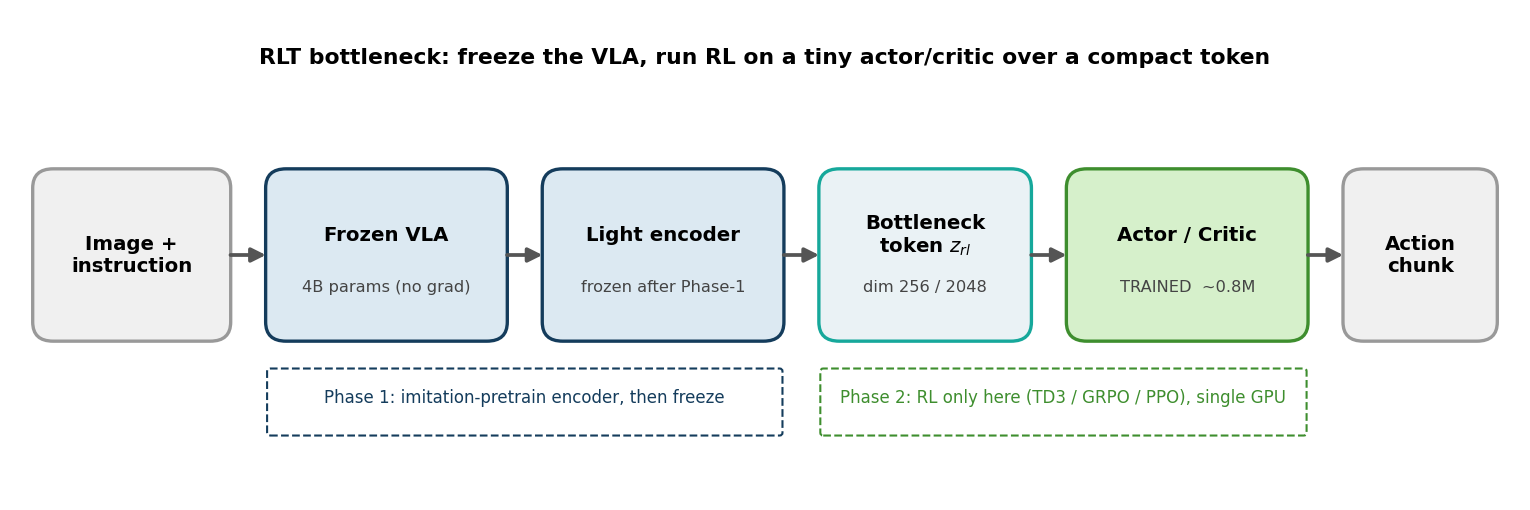
\includegraphics[width=\linewidth]{figures/rlt_architecture.png}
    \caption{\textbf{The RLT bottleneck.} The VLA and the light encoder are \emph{frozen}; RL trains only a tiny ($\sim$$0.8$\,M) actor/critic over a compact bottleneck token $z_{rl}$. Phase 1 imitation-pretrains the encoder and freezes it; Phase 2 runs RL (TD3/GRPO/PPO) on the bottleneck only, on a single GPU with no model parallelism.}
    \label{fig:rlt_arch}
\end{figure}

\textbf{Positioning (honest disclosure).} We do \emph{not} claim RLT is the global ceiling: a properly scaled full-VLA recipe (RLinf-VLA~\citep{rlinfvla2025}: OpenVLA-OFT~\citep{kim2025openvlaoft} + FSDP + 256 vectorized environments + DAPO-style GRPO) reaches $0.988$ on LIBERO-Goal, above our best RLT cell ($0.953$, $3$-seed). To make this comparison first-party and reproducible rather than citation-only, we additionally implement a \emph{faithfully scaled} full-VLA baseline of our own---FSDP across $6$ GPUs, all-$10$-task joint optimization, RLinf-aligned hyper-parameters and batch ($\sim$$720$ transitions/update)---which reaches $\mathbf{0.922}$ with PPO (\cref{tab:rlt_cost}). Two findings sharpen the picture: \textbf{(i) RLT$+$PPO ($0.953$, a single GPU) \emph{exceeds} this scaled $6$-GPU full-VLA PPO ($0.922$)}, so the bottleneck is not merely cheaper but more effective than faithful full-VLA RL at our scale; and \textbf{(ii) the full-VLA GRPO gap is mainly credit-assignment, not just GPU count}---scaling vanilla GRPO barely moves it ($0.740{\to}0.744$), while adding token-level log-prob credit plus temporal reward redistribution raises it to $0.796$ on one GPU and $0.836$ with FSDP-$5$ at iter-$150$ (offline $50$-ep). This still trails PPO, but it shows RLinf-style fine-grained credit is the useful ingredient; naive learning-rate alignment to RLinf (lr$=10^{-4}$) diverged in our setting. RLT's contribution is thus an \emph{order-of-magnitude cheaper} path that is algorithm-agnostic, stable, and competitive with---indeed above---faithfully scaled full-VLA RL at a fraction of its cost (\cref{tab:rlt_cost}).

\subsection{Systems and Implementation}
\label{sec:rlt_impl}
The platform's online-RL stage is engineered for low cost and robustness; the design choices below are as much systems as algorithmic, and are what let this stage run on commodity hardware.
\begin{itemize}[leftmargin=1.3em,itemsep=2pt,topsep=2pt]
  \item \textbf{Single-GPU, frozen-backbone RL---no model parallelism.} The $4$\,B VLA and the $130$--$250$\,M encoder are frozen; only a $0.85$--$2.7$\,M actor/critic is trained. Training fits on \emph{one} GPU with no FSDP/Megatron/vLLM sharding---the gradient step is negligible and each iteration is rollout-bound, removing the entire model-parallel stack that large-scale full-VLA RL requires.
  \item \textbf{One algorithm-agnostic interface.} TD3, GRPO, and PPO are implemented against the \emph{same} frozen-bottleneck state and actor/critic API, so changing the RL algorithm is a flag rather than a rewrite; on-policy cold-start is handled uniformly by a residual actor ($\mu=\tilde a+\Delta$).
  \item \textbf{Pluggable VLA backbone.} The repository abstracts the frozen VLA behind a common hidden-state / action-query adapter, so swapping the backbone is a \emph{configuration flag}, not a reimplementation---even across fundamentally different architectures: QwenOFT (Qwen2.5-VL, autoregressive action head) and Pi$0.5$ (PaliGemma $+$ continuous flow-matching action head) run through the \emph{same} RLT encoder, actor/critic, rollout, and RL code, and we verify the full pipeline (Phase-1 pretrain $\to$ Phase-2 RL $\to$ offline eval) on both (\cref{tab:rlt_backbone}). This makes RLT a backbone-agnostic add-on rather than a model-specific recipe.
  \item \textbf{Efficient, fault-tolerant rollout.} A persistent subprocess env-pool reuses MuJoCo environments across iterations over socket-pair IPC (no pipe-buffer deadlock), with async rollout overlapping collection and updates. A robustness layer makes cheap multi-run training survive shared-cluster reality: BLAS-thread pinning removes the hidden CPU-load multiplier; a configurable worker timeout plus a per-worker restart \emph{circuit breaker} turn transient CPU-oversubscription / EGL / render faults into soft per-env drops instead of run-killing restart storms; and checkpoint resume (weights $+$ optimizer) lets an OOM-killed or preempted run continue from its last iteration rather than restart from scratch.
\end{itemize}
The gradient step is negligible---an iteration of full-VLA PPO is dominated by CPU rollout ($214$\,s, $88\%$, GPU $\sim$$1\%$) with only $30$\,s of $4$\,B-parameter update, whereas RLT updates a ${\sim}0.8$\,M actor/critic---so the stage is rollout-bound and one GPU suffices. Together these let the platform \emph{run and recover} VLA RL on a single commodity GPU at a small fraction of the engineering and compute cost of full-VLA fine-tuning. For a like-for-like reference point, the same codebase also implements the \emph{opposite} regime---a faithfully-scaled FSDP full-VLA RL path (multi-GPU \texttt{FULL\_SHARD}, all-task joint rollout, NCCL grad reduction), used for the first-party scaled baseline in \cref{tab:rlt_cost}---together with a shared-storage job agent for multi-machine orchestration, so the cheap and the scaled regimes are directly comparable within one implementation.

\subsection{Experimental Setup}
\label{sec:rlt_setup}

\textbf{Benchmark and protocol.} We evaluate on \textbf{LIBERO-Goal}~\citep{liu2023libero} ($10$ tasks). Unless noted, every number is an \emph{offline} re-evaluation of the final (iter-$300$) checkpoint with $50$ episodes/task (seed $42$, max $320$ low-level steps; success $=$ environment reward $\ge 0.5$ at termination)---never the noisy in-training $20$-episode monitor. We report task $0$/task $3$ (easy/hard) and the all-$10$-task mean.

\textbf{Bottleneck encoders.} Two variants compress the frozen VLA hidden state: \textbf{RLT} (full-token cross-attention, bottleneck dim $2048$) and \textbf{RLT$_a$} (action-query slice with an extra $H{\to}256$ projection; fewer parameters, tighter bottleneck). Each encoder is pretrained by offline imitation (reconstructing the VLA reference action) and then frozen for the RL stage.

\textbf{Algorithms and baselines.} On the bottleneck we run \emph{TD3} (off-policy actor-critic; BC-anchored actor), \emph{GRPO} (critic-free, group-relative advantage), and \emph{PPO} (GAE $+$ value). On-policy cold-start is fixed with a residual actor ($\mu=\tilde a+\Delta$). As baselines we directly RL the entire VLA (\emph{VLA$+$PPO}, \emph{VLA$+$GRPO}) in two regimes: a \emph{small-scale} implementation (few environments, micro-batch $2$, no FSDP) for compute-matched comparison, and a \emph{faithfully scaled} implementation we built for a first-party full-VLA upper-reference (FSDP across $6$ GPUs, all-$10$-task joint optimization, micro-batch $80$, RLinf-aligned learning rate and $\sim$$720$-transition update batch).

\subsection{Results and Analysis}
\label{sec:rlt_results}

\begin{table}[t]
    \centering
    \caption{\textbf{Main results on LIBERO-Goal (QwenOFT-5traj base, offline 50-ep, iter-300).} Success rate ($\uparrow$). All cells verified against source eval JSON. \textsc{All-10} is the all-$10$-task mean; \textsc{Task 0}/\textsc{Task 3} are easy/hard single tasks. All-task cells are the $3$-seed (42/43/44) mean; the per-route spread is small (all-task std $\le 0.05$, largest for GRPO at $0.05$), so we report point estimates here and show the std bands in \cref{fig:rlt_convergence}. Best all-task in \textbf{bold} (the two PPO routes are tied). The scaled FSDP-$6$ VLA$+$PPO row is offline 50-ep at iter-$300$ (all-$10$-task joint, RLinf-aligned hyper-parameters); even on $6$ GPUs it lands below RLT$+$PPO.}
    \label{tab:rlt_main}
    \vspace{0.3em}
    \footnotesize
    \setlength{\tabcolsep}{6pt}
    \renewcommand{\arraystretch}{1.18}
    \begin{tabular}{@{}l l ccc@{}}
        \toprule
        \textbf{Method} & \textbf{Encoder} & \textsc{Task 0} & \textsc{Task 3 (hard)} & \textsc{All-10} \\
        \midrule
        \rowcolor{abMist} Base VLA (pre-RL) & ---     & 0.78 & 0.42 & 0.704 \\
        RLT $+$ TD3       & RLT    & 0.98 & 0.64           & 0.830 \\
        RLT $+$ GRPO      & RLT    & 0.96 & 0.71 & 0.786 \\
        \textbf{RLT $+$ PPO} & RLT & 0.94 & \textbf{0.95} & \textbf{0.953} \\
        RLT$_a$ $+$ TD3   & RLT$_a$& 0.82 & 0.46           & 0.920 \\
        RLT$_a$ $+$ GRPO  & RLT$_a$& 0.88 & 0.70           & 0.753 \\
        \textbf{RLT$_a$ $+$ PPO} & RLT$_a$ & \textbf{1.00} & 0.96 & \textbf{0.951} \\
        \midrule
        VLA $+$ PPO (small-scale, ours)  & --- & 0.96 & 0.80 & 0.718 \\
        VLA $+$ GRPO (small-scale, ours) & --- & 0.80 & 0.62 & 0.756 \\
        VLA $+$ PPO (scaled FSDP-6, ours) & --- & 1.00 & 0.78 & 0.922 \\
        \bottomrule
    \end{tabular}
\end{table}

\begin{figure}[t]
    \centering
    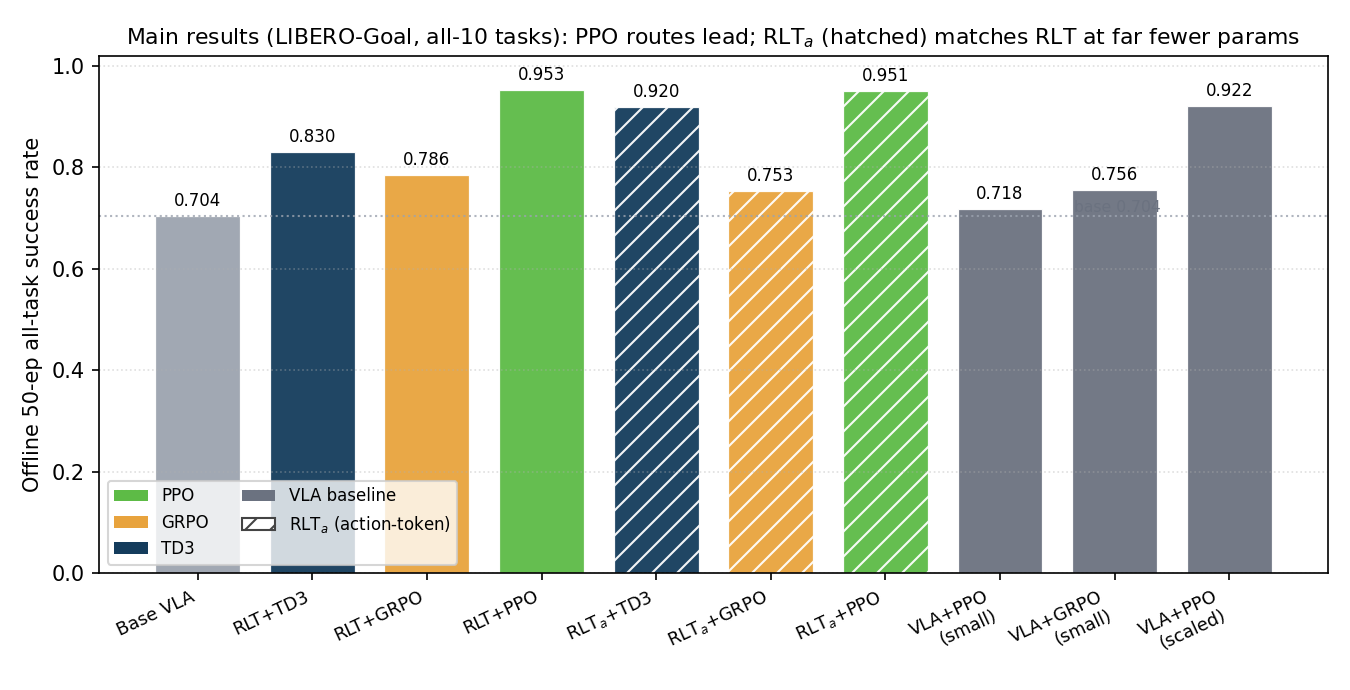
\includegraphics[width=0.95\linewidth]{figures/rlt_main_bar.png}
    \caption{\textbf{Main results (all-10-task SR).} The two PPO routes (green) lead at ${\sim}0.95$; GRPO and TD3 sit lower; the small-scale VLA baselines (gray) are near the SFT base. Hatched bars are the action-token RLT$_a$ variant---it tracks full-token RLT at $3\times$ fewer trained parameters.}
    \label{fig:rlt_mainbar}
\end{figure}

\textbf{(RQ-A) The bottleneck is an algorithm-agnostic interface.} All three RL algorithms plug into the frozen-VLA bottleneck and improve over the base policy ($0.704\!\to\!0.79$--$0.95$ all-task, $3$-seed). The \textbf{two PPO routes are the strongest and essentially tied} (RLT$+$PPO $0.953$, RLT$_a$$+$PPO $0.951$), well above our GRPO ($0.786$). \emph{This ordering is specific to our \textbf{vanilla} GRPO (basic group-relative advantage, $\le2$ groups/state, no enhancements) at small scale---not an algorithmic ceiling}: RLinf's enhanced \textbf{DAPO-GRPO} (clip-higher, dual-clip, valid-action masking, success-rate dynamic filtering, group-size $8$, $256$ environments) reaches $0.988$ on this benchmark, on par with the best PPO. We verified this diagnosis inside our codebase: scaling vanilla full-VLA GRPO alone leaves it at $0.744$, but adding token-level log-prob credit and temporal return redistribution raises the same stack to $0.796$ (single GPU, iter-$300$) and $0.836$ (FSDP-$5$, iter-$150$), both from offline $50$-episode evaluation. Thus the GRPO gap below reflects missing fine-grained credit machinery more than a categorical weakness of GRPO. On easy/saturated tasks the algorithms are within noise; on the \emph{hard} task $3$ they separate sharply: $\text{PPO}\gg\text{GRPO}\approx\text{TD3}$ ($0.95$ vs $0.71/0.64$). Mechanistically, under sparse reward TD3's BC anchor limits exploration and critic-free GRPO often sees a zero-signal group, whereas PPO's per-state GAE value signal best guides exploration---a conclusion that holds on both encoders ($t_3=0.95$ for RLT, $0.96$ for RLT$_a$), indicating an algorithm property rather than an encoder artifact. \Cref{fig:rlt_convergence} traces the full encoder$\times$algorithm matrix from a cold start: both PPO routes climb fastest and plateau highest ($\sim0.92$--$0.95$), GRPO plateaus low and flat ($\sim0.72$--$0.75$), and off-policy TD3 rises more slowly and noisily to $0.83$---the algorithm ordering is consistent across the two encoders, and every route learns from an untrained ($0$ success) actor.

\begin{figure}[t]
    \centering
    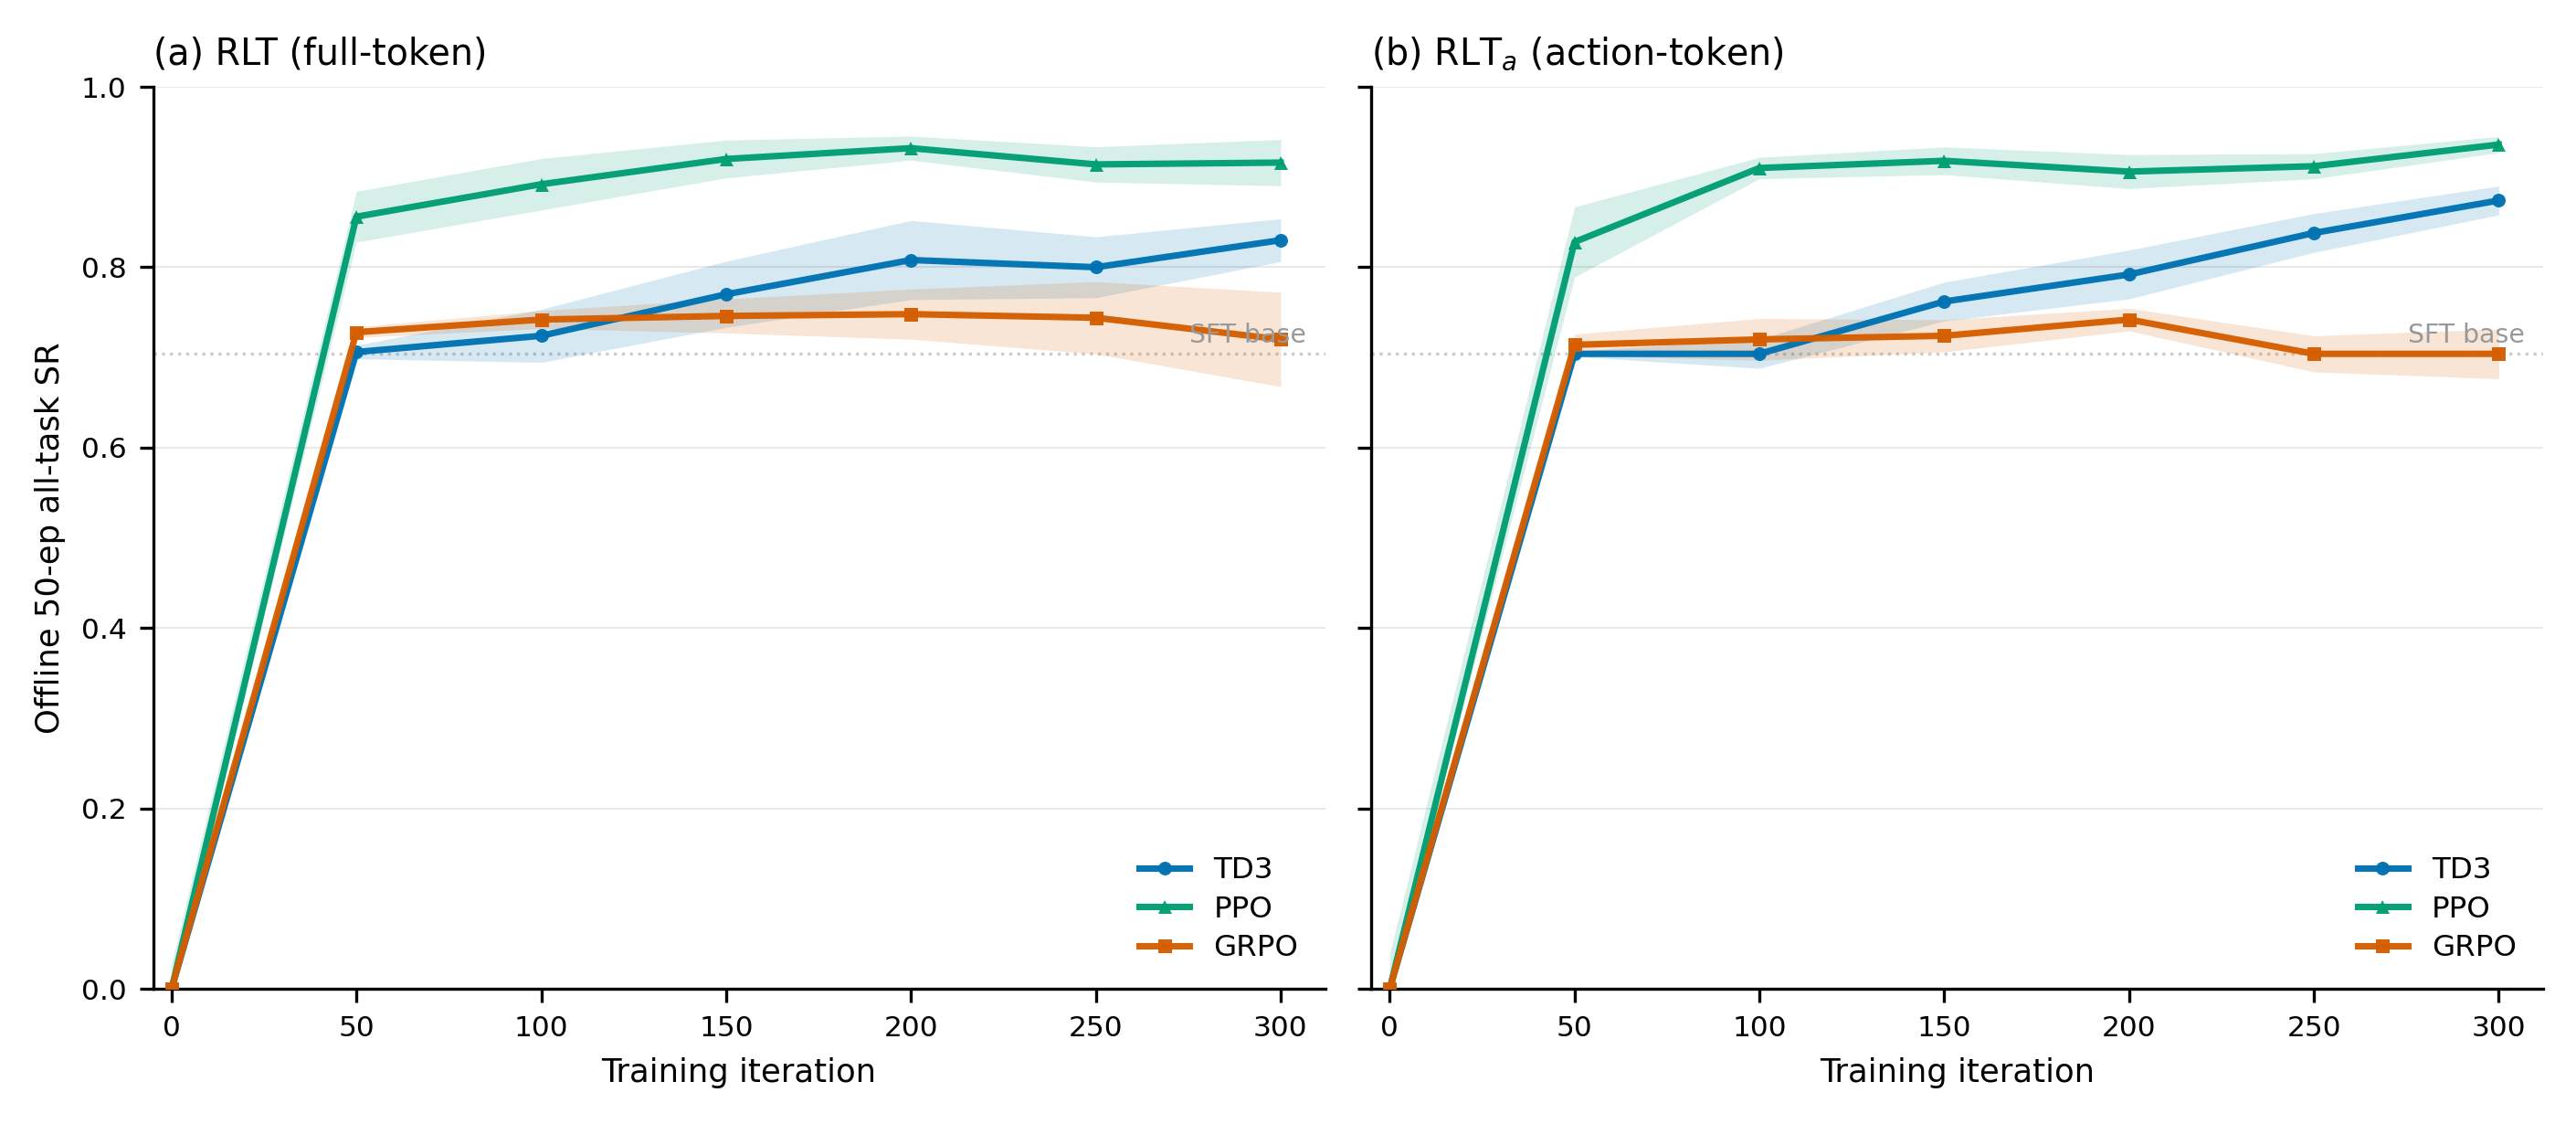
\includegraphics[width=\linewidth]{figures/rlt_convergence_panels.png}
    \caption{\textbf{Convergence of the six RLT routes (encoder $\times$ algorithm), single GPU, cold start.} Offline 50-ep all-task success rate vs.\ training iteration. Color $=$ algorithm (TD3 navy / PPO green / GRPO amber); linestyle $=$ encoder (solid $=$ RLT full-token, dashed $=$ RLT$_a$ action-token). All curves start at iter $0=0$: the residual actor is untrained at initialization, so RL learns from scratch on top of the frozen backbone. Both PPO routes plateau highest, GRPO lowest, TD3 in between and noisiest. Shaded bands show the multi-seed std ($n\ge2$) for the routes with seed reruns.}
    \label{fig:rlt_convergence}
\end{figure}

\textbf{(Encoder design) RLT$_a$ is the compact sweet spot: near-identical accuracy at ${\sim}3\times$ fewer trained parameters.} The two encoders trade accuracy against compactness (\cref{tab:rlt_encoder}). Full-token RLT keeps the VLA's full $2048$-dim hidden width as its bottleneck; action-token RLT$_a$ instead reads only the VLA's \emph{action-query} slice---which already concentrates the action-relevant information---and projects it to a $256$-dim bottleneck ($8\times$ narrower). Because the actor/critic consume the bottleneck directly, this narrower interface cascades into a $3.2\times$ smaller trainable head ($0.85$\,M vs $2.68$\,M actor$+$critic; the entire per-layer saving is in the input projection, $512{\times}312$ vs $512{\times}2104$) and a $1.8\times$ smaller frozen encoder ($135$\,M vs $248$\,M). Yet RLT$_a$+PPO \emph{matches} RLT+PPO on the all-task mean (near-identical, $0.951$ vs $0.953$) and is the single strongest \emph{single-task} cell ($t_0/t_1/t_3=1.00/0.98/0.96$ vs $0.94/0.92/0.95$); the bottleneck-dimension ablation ($D{=}128/256/512$ all ${\sim}0.82$--$0.84$) confirms the tight bottleneck is not fragile. \textbf{Practical takeaway: use RLT+PPO ($0.953$) for the highest absolute success rate, or RLT$_a$+PPO for an ${\sim}3\times$ lighter model at the same accuracy.}

\begin{table}[t]
    \centering
    \caption{\textbf{Encoder design: full-token RLT vs.\ action-token RLT$_a$ (PPO).} The action-query slice $+$ tight $256$-dim bottleneck yields ${\sim}3\times$ fewer trainable parameters at near-identical accuracy. Param counts measured from checkpoints; SR offline 50-ep.}
    \label{tab:rlt_encoder}
    \vspace{0.3em}
    \footnotesize
    \setlength{\tabcolsep}{7pt}
    \renewcommand{\arraystretch}{1.15}
    \begin{tabular}{@{}l cc@{}}
        \toprule
        & \textbf{RLT} (full-token) & \textbf{RLT$_a$} (action-token) \\
        \midrule
        Bottleneck dim            & $2048$            & $256$ ($8\times$ narrower) \\
        Trainable (actor$+$critic)& $2.68$\,M         & $\mathbf{0.85}$\,M ($3.2\times$ fewer) \\
        Frozen encoder            & $247.6$\,M        & $135.4$\,M \\
        \midrule
        All-10 (PPO)              & $0.953$ & $0.951$ \\
        Single-task $t_0/t_1/t_3$ & $0.94/0.92/0.95$  & $\mathbf{1.00/0.98/0.96}$ \\
        \bottomrule
    \end{tabular}
\end{table}

\begin{figure}[t]
    \centering
    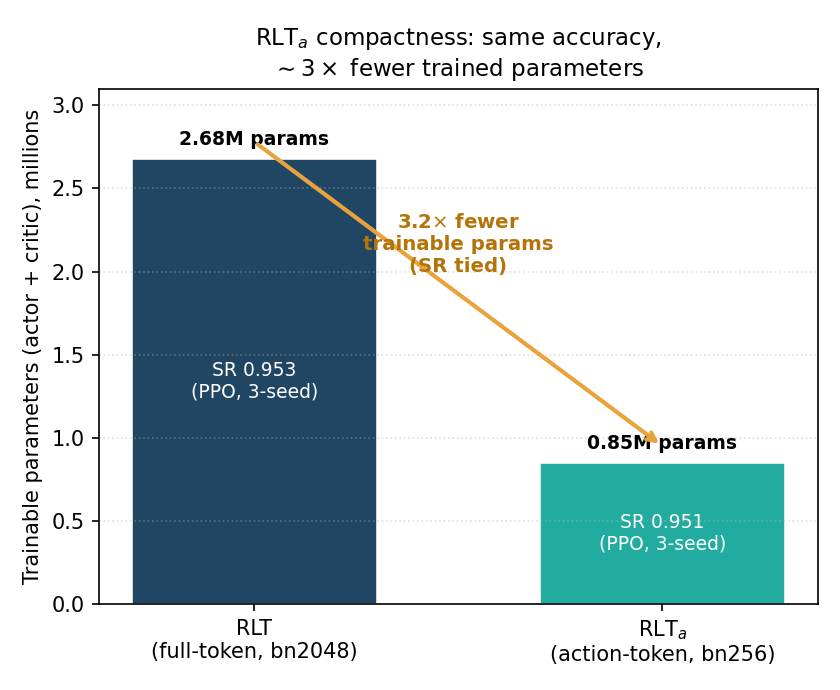
\includegraphics[width=0.56\linewidth]{figures/rlt_param_efficiency.png}
    \caption{\textbf{RLT$_a$ compactness.} The action-token encoder trains a $3.2\times$ smaller actor/critic ($0.85$\,M vs $2.68$\,M) for a near-identical all-task success rate ($0.951$ vs $0.953$, PPO).}
    \label{fig:rlt_parameff}
\end{figure}

\textbf{(RQ-B) Efficiency, not success-rate supremacy.} Against our own small-scale full-VLA baselines, the RLT route is higher and far more stable: across the 1-traj single-task runs the VLA baselines' online SR swings wildly (VLA$+$PPO task-0 over 15 evals spans $55$--$100\%$, VLA$+$GRPO $35$--$75\%$) versus RLT's tight band (task-0 $85$--$100\%$, std $<5$), and the offline VLA$+$PPO 5-traj curve rises to $0.798$ then decays to $0.71$. However, this is a \emph{compute-matched} comparison: our VLA baselines are under-scaled. The defensible claim is cost (\cref{tab:rlt_cost}): RLT reaches $0.953$ on \emph{one} GPU ($\sim$$55$--$69$\,GB, frozen $4$\,B VLA $+$ batched rollout), training only ${\sim}0.8$\,M actor/critic parameters ($<0.02\%$, no FSDP), whereas large-scale full-VLA RL (RLinf-VLA) reaches $0.988$ with $8{+}$ GPUs of FSDP, ${\sim}640$\,GB total, the full $4.1$\,B parameters, and $256$ environments. RLT thus trades ${\sim}8\times$ fewer GPUs, ${\sim}5000\times$ fewer trainable parameters ($0.8$\,M vs $4.1$\,B), and no model-parallel infrastructure for ${\sim}96\%$ of the absolute success rate. Crucially, this efficiency does \emph{not} cost effectiveness relative to \emph{faithful} full-VLA RL: our own scaled VLA$+$PPO (FSDP-$6$, all-$10$-task, RLinf-aligned) reaches $0.922$, still \emph{below} RLT$+$PPO's $0.953$---so the single-GPU bottleneck is at least as strong as $6$-GPU full-parameter fine-tuning at a fraction of the cost, and the remaining gap to RLinf is closed by RLinf's algorithmic additions (DAPO clip-higher, partial-reset, valid-action masking, $256$ environments) rather than by scaling our recipe (an aligned lr$=10^{-4}$ run diverged within two iterations). We further verified that the residual gap to RLinf is \emph{not} a measurement artifact: re-evaluating our VLA baselines under RLinf's lenient \emph{success-once} criterion shifts them by only ${\pm}2$\,pp (PPO $0.718{\to}0.74$, GRPO $0.756{\to}0.75$), so the distance to RLinf's $0.988$ is dominated by training scale rather than the success definition. \Cref{fig:rlt_vs_vla} makes the cold-start contrast explicit: the best RLT route (RLT$_a$+PPO, $\sim0.8$\,M trained parameters, one GPU) begins from $0$ and overtakes our small-scale full-VLA baselines, which start from the $0.704$ SFT head-start yet stagnate (VLA$+$GRPO) or peak-and-decay (VLA$+$PPO, $0.80\!\to\!0.71$).

\begin{figure}[t]
    \centering
    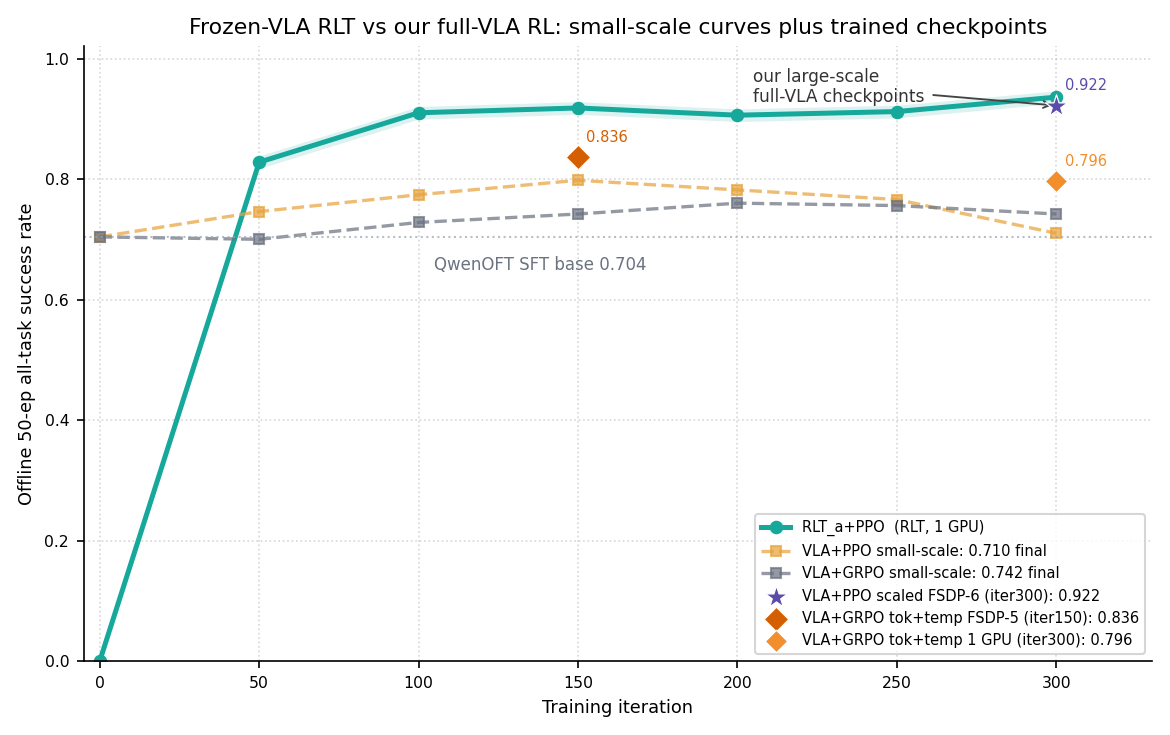
\includegraphics[width=0.78\linewidth]{figures/rlt_vs_vla_curve.png}
    \caption{\textbf{Frozen-VLA RLT vs.\ our full-VLA RL.} Offline 50-ep all-task success rate per checkpoint. RLT$_a$+PPO (teal) learns from a cold $0$ and overtakes our small-scale full-VLA baselines (dashed), which begin from the measured $0.704$ SFT base. The same plot overlays our trained large-scale full-VLA checkpoints without drawing artificial endpoint lines: scaled FSDP-$6$ VLA$+$PPO ($0.922$ at iter-$300$), token-level+temporal-credit VLA$+$GRPO on FSDP-$5$ ($0.836$ at iter-$150$), and the matching single-GPU token-level+temporal-credit VLA$+$GRPO run ($0.796$ at iter-$300$).}
    \label{fig:rlt_vs_vla}
\end{figure}

\begin{table}[t]
    \centering
    \caption{\textbf{Resource comparison: RLT (ours) vs.\ faithfully-scaled full-VLA RL (ours) vs.\ RLinf-VLA.} RLT and our scaled-VLA numbers are measured first-party (per-PID GPU memory; trainable params from checkpoint sizes; our scaled VLA$+$PPO is FSDP-$6$, all-$10$-task, RLinf-aligned hyper-parameters, offline 50-ep); the RLinf-VLA column is its reported $8$-GPU FSDP configuration~\citep{rlinfvla2025}. \textbf{RLT$+$PPO on one GPU exceeds our $6$-GPU scaled full-VLA PPO.}}
    \label{tab:rlt_cost}
    \vspace{0.3em}
    \footnotesize
    \setlength{\tabcolsep}{6pt}
    \renewcommand{\arraystretch}{1.18}
    \begin{tabular}{@{}l ccc@{}}
        \toprule
        & \textbf{RLT (ours)} & \textbf{Scaled VLA (ours)} & \textbf{RLinf-VLA} \\
        \midrule
        Trainable parameters     & $\sim$$0.8$\,M & $\sim$$4.1$\,B (FSDP) & $\sim$$4.1$\,B (FSDP) \\
        Trainable fraction       & $<0.02\%$ & $100\%$ & $100\%$ \\
        Training GPUs            & \textbf{1} & $6$ (FSDP) & $8{+}$ (FSDP) \\
        GPU memory               & $\sim$$55$--$69$\,GB & $6{\times}80$ & $\sim$$640$\,GB ($8{\times}80$) \\
        Parallel environments    & $4$--$8$ & $120$ (all-task) & $128$--$256$ \\
        Backend                  & single-process & FSDP (ours) & FSDP $+$ vLLM/Megatron \\
        \midrule
        LIBERO-Goal SR           & $\mathbf{0.953}$ & $0.922$ & $0.988$ \\
        \bottomrule
    \end{tabular}
\end{table}

\textbf{(RQ-C) Failure boundary.} With weak data ($1$-trajectory base), the hard task collapses \emph{method-agnostically}: base $t_3=0.00$, and after RL the released RLT$_a$$+$TD3 cell shows negative transfer ($0.08$) while the VLA baselines also fail. The gap is data-driven, not architecture-driven (QwenOFT $5$-traj vs $1$-traj all-task: $0.920$ vs $0.548$, with the difference concentrated entirely on hard tasks). Even here, the PPO hard-task advantage persists: on the 1-traj base (task-3 base $=0.00$), RLT$+$PPO reaches $0.80$ while RLT$+$GRPO ($0.08$), RLT$+$TD3 ($0.12$), and both VLA baselines all fail to exceed $\sim0.12$---so among all methods only PPO learns the hard task in the data-scarce regime.

\textbf{(RQ-D) Cross-backbone.} Enabled by the pluggable-backbone interface (\cref{sec:rlt_impl}), the \emph{same} RLT pipeline transfers from QwenOFT to Pi$0.5$ (PaliGemma $+$ flow-matching) with only a configuration change (\cref{tab:rlt_backbone}). With RLT$+$TD3, Pi$0.5$-5traj reaches $0.868$ all-task ($>$ QwenOFT $0.830$) and is actually stronger on the hard single task ($t_3$ $0.82$ vs $0.64$), indicating the RL gain couples to the backbone's weak skills and decouples from the backbone family.

\begin{table}[t]
    \centering
    \caption{\textbf{Cross-backbone (RLT $+$ TD3, 5-traj).} Offline 50-ep. Single-task $t_0/t_1/t_3$ and all-10-task mean. The \emph{same} RLT pipeline runs on both backbones via a config flag; Pi$0.5$ even edges out QwenOFT.}
    \label{tab:rlt_backbone}
    \vspace{0.3em}
    \footnotesize
    \setlength{\tabcolsep}{7pt}
    \renewcommand{\arraystretch}{1.15}
    \begin{tabular}{@{}l l ccc c@{}}
        \toprule
        \textbf{Backbone} & \textbf{Data} & \textsc{T0} & \textsc{T1} & \textsc{T3} & \textsc{All-10} \\
        \midrule
        QwenOFT & 5-traj & 0.98 & 0.92 & 0.64 & 0.830 \\
        Pi0.5   & 5-traj & 0.98 & 1.00 & \textbf{0.82} & \textbf{0.868} \\
        \bottomrule
    \end{tabular}
\end{table}

\textbf{(RQ-E) Ablations} (RLT$+$TD3, task $0$): Phase-1 encoder pretraining is essential ($0.98\!\to\!0.66$ when randomly initialized, $-0.32$); the BC-anchor regularizer is the lifeline of off-policy RL under sparse reward ($\beta{=}0\!\Rightarrow\!0.00$); the bottleneck dimension is robust ($D{=}128/256/512$ all ${\sim}0.82$--$0.84$).

\textbf{Per-task algorithm matrix (single-task).} Beyond the all-task means, the single-task matrix (\cref{tab:rlt_algo}) isolates the algorithm $\times$ difficulty interaction on a fixed RLT encoder. The three algorithms tie on easy/medium tasks ($0.92$--$0.98$); the separation is entirely on the hard task $3$, where PPO's $0.95$ is the single best RLT result and the only algorithm to reliably solve it.

\begin{table}[t]
    \centering
    \caption{\textbf{RLT $\times$ RL algorithm, single-task LIBERO-Goal} (fixed RLT encoder, offline 50-ep, iter-300). Point estimates; multi-seed spread is small ($<0.05$, shown in \cref{fig:rlt_convergence}).}
    \label{tab:rlt_algo}
    \vspace{0.3em}
    \footnotesize
    \setlength{\tabcolsep}{8pt}
    \renewcommand{\arraystretch}{1.15}
    \begin{tabular}{@{}l l ccc@{}}
        \toprule
        \textbf{Algorithm} & \textbf{Type} & \textsc{Task 0} & \textsc{Task 1} & \textsc{Task 3 (hard)} \\
        \midrule
        TD3  & off-policy AC (twin-$Q$)      & \textbf{0.98} & 0.92 & 0.64 \\
        GRPO & on-policy, critic-free        & 0.96 & \textbf{0.96} & 0.71 \\
        PPO  & on-policy AC (GAE)            & 0.94 & 0.92 & \textbf{0.95} \\
        \bottomrule
    \end{tabular}
\end{table}

\textbf{Training dynamics and data scaling.} The online success rate is noisy across iterations (e.g.\ RLT$+$TD3 on task $0$ oscillates in $0.74$--$0.92$ over iters $150$--$300$); we therefore select the model by the mean of the last three checkpoints rather than the peak, and report all headline numbers from a uniform \emph{offline} 50-ep re-evaluation. RL gains are strongly \emph{data-volume}-dependent: the released RLT$_a$$+$TD3 all-task cell drops from $0.920$ (5-traj base) to $0.548$ (1-traj base), and the $0.372$ gap is concentrated entirely on hard/long-horizon tasks (e.g.\ $t_9$ $+0.90$, $t_5$ $+0.82$), while easy tasks are within $0.08$---consistent with the sparse-reward failure boundary of RQ-C.

\subsection{Summary}
The RLT bottleneck is the platform's algorithm-agnostic, single-GPU, $<0.1\%$-trainable-parameter interface for online VLA RL. PPO is the clear best algorithm on it (top accuracy \emph{and} hardest-task and sample efficiency), with \textbf{RLT$+$PPO reaching the highest absolute success rate ($0.953$)}. The two encoder variants give a clean accuracy/compactness choice: \textbf{the action-token RLT$_a$ matches full-token RLT's accuracy ($0.951$, tied) at ${\sim}3\times$ fewer trainable parameters and an $8\times$ narrower bottleneck}, because the VLA's action-query slice already concentrates the action-relevant signal. The overall value of RLT is the performance/cost ratio and training stability: on a \emph{single} GPU it \emph{exceeds} our own faithfully-scaled $6$-GPU full-VLA PPO ($0.953$ vs $0.922$) and reaches ${\sim}96\%$ of large-scale RLinf-VLA's $0.988$ at ${\sim}1/8$ the GPUs and ${\sim}5000\times$ fewer trainable parameters---the residual gap being RLinf's algorithmic additions (DAPO, partial-reset, valid-action masking) rather than scale, since naively aligning our learning rate to RLinf's diverged.



\begin{thebibliography}{9}
\bibitem{liu2023libero} B.~Liu et al. {LIBERO}. NeurIPS 2023.
\bibitem{rlinfvla2025} RLinf Team. {RLinf-VLA}. arXiv:2510.06710, 2025.
\bibitem{rltoken2026} RL Token Authors. {RL Token}. arXiv preprint, 2026.
\bibitem{fujimoto2018td3} S.~Fujimoto et al. TD3. ICML 2018.
\bibitem{schulman2017ppo} J.~Schulman et al. PPO. arXiv:1707.06347, 2017.
\bibitem{shao2024grpo} Z.~Shao et al. DeepSeekMath (GRPO). arXiv:2402.03300, 2024.
\bibitem{kim2025openvlaoft} M.~J.~Kim et al. OpenVLA-OFT. arXiv:2502.19645, 2025.
\end{thebibliography}\end{document}
